\chapter{Wnioski}
\label{c6}

\section{Zalety programowania wizualnego}

Główną zaletą programowania wizualnego jest łatwość, z jaką przychodzi pisać aplikacje. Nie trzeba być doświadczonym programistą, aby tworzyć aplikacje za pomocą App Inventora. Jeżeli ktoś jest zainteresowany programowaniem i nie wie jak zacząć, programowanie wizualne może okazać się dobrym wyborem na start. Nauka programowania wizualnego nie jest skomplikowana, wystarczą chęci. 

Kolejną zaletą jest nieskomplikowany sposób stworzenia dobrze wyglądającego interfejsu graficznego (\english{GUI}). Nie znać języku XML aby zdefiniować ładny układ i wygląd ekranu. Wszystkie elementy są przeciągane z palety komponentów, a ich właściwości ustawiane również w prosty sposób.

Następną zaletą są możliwości jakie daje programowanie wizualne. Mimo, że wiele funkcji nie jest dostępnych to aplikacje, które można stworzyć za pomocą App Inventora mogą być bardzo rozbudowane. Komponenty oferowane przez to środowisko pokrywają zdecydowaną większość podstawowych i najbardziej używanych elementów, których się używa podczas pisania aplikacji w języku Java. Jeżeli jakiegoś komponentu brakuje, np. przycisków typu Radio, w internecie jest wiele materiałów w jaki sposób można to obejść.

Myślenie wizualne jest bardziej naturalne dla człowieka. Programowanie w App Inventorze daje programistom możliwość pisania programów poprzez manipulację elementami graficznymi. Dopiero doświadczony programista będzie potrafił sobie wyobrazić na wyższym poziomie abstrakcji kod tekstowy. Dlatego też kod aplikacji Javowej musi spełniać założenia wzorców projektowych, dzięki czemu łatwość nawigowania pomiędzy klasami i metodami jest dużo większa. W App Inventorze stworzenie zadanej funkcjonalności sprowadza się zwykle do użycia pojedynczych bloków, co daje dużą przejrzystość. Dopiero skomplikowane aplkiacje mogłyby rozrosnąć się, tak że zrozumienie ich zajełoby dużo więcej czasu niż takiej samej aplikacji napisanej w języku Java. Jednak jeżeli jest to tak skompilkowana aplikacja warto się zastanowić czy napisanie jej w App Inventorze to dobry pomysł.

App Inventor może być również dobrym narzędziem do tworzenia prototypów. Aplikacje tworzone za pomocą niego powstają bardzo szybko. Stworzony układ graficzny można w krótkim czasie zaprezentować biznesowi, który dzięki temu będzie miał szansę szybko zareagować i skorygować lub zatwierdzić dany interfejs.

\section{Wady programowania wizualnego}

Przynajmniej na razie nie ma możliwości rozszerzenia App Inventora, więc jeżeli istniałaby potrzeba stworzenia lub skorzystania z czegoś, co nie jest wbudowane bezpośrednio w oferowaną platformę, jak np. grafika 3D, to ostatecznie okaże się że projekt nie zostanie zrealizowany.

Implementacja App Inventora nie jest zoptymalizowana dla gier o wysokiej wydajności. Cały framework App Inventora zużywa o wiele więcej mocy procesora, niż programy napisane w języku Java. Przy zwykłym sortowaniu program napisany w Javie jest średnio 2 tysiące razy szybszy.

Stworzenie większego projektu i decyzja o użyciu App Inventora pociąga za sobą zaangażowanie wielu programistów. Nie mogą oni jednak pracować współbieżnie. Współdzielenie projektu odbywa się na zasadzie wyeksportowania go na komputer jako spakowane archiwum. Następnie kolejny programista może go zaimportować. Nie ma to jednak większego sensu, ponieważ kiedy dwie osoby będą pracować nad tym samym projektem, nie będzie można go na końcu scalić. Odwrotnie jest przy pisaniu aplikacji w języku natywnym. Istnieje bardzo wiele narzędzi do rozwiązania tego problemu, są to tzw. systemy zarządzania wersją kodu (\english{Source code management systems}).

\subsection{Inne ograniczenia App Inventora}

\begin{itemize}
\item Animacja nie jest wspierana automatycznie. Jeżeli programista chciałby stworzyć animowany GIF, posiadając kilka różnych obrazków, z których ten GIF miałby się składać, musi zrobić to manualnie. Zautomatyzowanie tego procesu byłoby bardzo pomocne.\cite{android:57}
\item App Inventor nie wspiera gestów multi-touch, czyli dotykania ekranu i wykonywanie czynności kilkoma palacmi w jednym momencie.\cite{android:57}
\item Brak wsparcia dla rysowania obrazków o standardowych kształtach. Są to między innymi prostokąty, trójkąty, koła, tekst. Programista chcąc dodać nowy element musi najpierw go stworzyć ręcznie a następnie wysłać na serwer App Inventora.\cite{android:57}
\item Niemożliwe jest tworzenie widżetów. App Inventor nie wspiera danej funkcji
\end{itemize}


\subsection{Podsumowanie}


App Inventor to sposób pomocy dla kogoś, kto nie miał styczności z programowaniem. Ogólnie rzecz biorąc istnieje kompromis pomiędzy programowaniem wizualnym, a programowaniem natywnym jeżeli chodzi o łatwość użycia, a ekspresywność i moc jaką daje znajomość Javy. Napisanie prostego \emph{Hello World} jest zazwyczaj łatwiejsze w środowiskach oferujących programowanie wizualne. W języku Java, który ma bardzo wiele zastosowań, aby stworzyć i zrozumieć prosty program wyświetlający napis \emph{Hello World} trzeba poznać wiele elementów Javy. Są to między innymi klasy, metody statyczne, pakiety, wywołania metod, różne strumienie do wyświetlenia danego tekstu, składnia języka. Jak widać jest to bardzo dużo elementów. 

Jednym z przykładów, który sprawia, że App Inventor jest nastawiony na początkujących programistów jest numerowanie list od 1, zamiast od 0, co może wydawać się nieintuicyjne dla doświadczonych programistów. Głównie to co sprawia że programowanie wizualne jest nastawione na początkujących jest eliminacja możliwości popełnienia błędów składniowych, uniemożliwiając tym samym stworzenie niedziałających programów. 

Z drugiej strony stworzenie prostej funkcji wielomianowej: $4x^3+2x^2-5x+1$ może okazać się bardziej czasochłonne niż napisanie jej w Javie. 
Na poniższych rysunkach widać, że funkcja napisana w Javie może okazać się łatwiejsza w zrozumieniu.


\begin{figure}[H]
\centering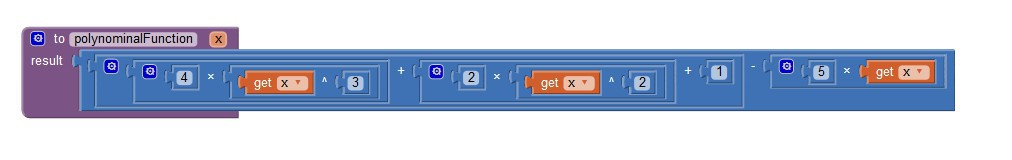
\includegraphics[width=15cm]{figures/polynominalFunction}
\caption{Bloki tworzące powyższą funkcję wielomianową}
\end{figure}

\begin{lstlisting}
int polynominalFunction(int x){
	return (int)(4*pow(x,3)+2*pow(x,2)-5*x+1);
}
\end{lstlisting}


Podsumowując można stwierdzić, że niektóre gry, takie jak quizy dadzą się zaimplementować za pomocą App Inventora. Natomiast gdy potrzebujemy płynnej animacji i stojącej za nią bardziej skomplikowanej logiki powinniśmy skorzystać z SDK, które oferuje nam Android. Języki blokowe wydają się być przeznaczone dla początkujących, więc projekty nie są tak zaawansowane, jak te, które są stworzone w języku natywnym. Korzystanie z bloków i przeciąganie ich jest nieporęczne dla złożonych programów.

Język wizualny jest przydatny, jeżeli programista ma na myśli proste projekty. Zawodzą one natomiast, jeżeli chodzi o zarządzanie na wielu poziomach abstrakcji i ziarnistości, jaką wymagają duże projekty. Mają one szansę odnieść sukces jako narzędzie, które będzie wyspecjalizowane w konkretnej domenie. System Android bardzo szybko rozrasta się i często pojawiają się nowe dostępne funkcjonalności. App Inventor jest narzędziem, który potrafi wykorzystać podstawowe, komponenty systemu Android, skupiając się na początkujących programistach. Jego celem nie są doświadczone osoby programujące od wielu lat, ponieważ, będą one chciały skorzystać z funkcji, które nie są dostępne.

Z drugiej strony można zauważyć, że programowanie wizualne jest coraz bardziej popularne. Główne środowiska programistyczne używane przez programistów Javy np. Intellij, Eclipse posiadają graficzne wtyczki umożliwiające tworzenie interfejsu poprzez przeciąganie komponentów. Nie są one idealne, jednak o wiele łatwiej jest z nich skorzystać, a następnie zmienić wygenerowany kod odpowiadający za wygląd ekranu.





